\input{configuration}

\title{Lecture 18 --- Query Evaluation and Optimization}

\author{Jeff Zarnett \\ \small \texttt{jzarnett@uwaterloo.ca}}
\institute{Department of Electrical and Computer Engineering \\
  University of Waterloo}
\date{\today}


\begin{document}

\begin{frame}
  \titlepage

 \end{frame}
 
\begin{frame}
\frametitle{Query Evaluation}

The strategies we have looked at thus far have explained how to perform individual parts of a query. 

If a simple select statement or a select-join is needed then we just have to carry it out using an evaluation plan. 

\begin{center}
	
\includegraphics[width=0.3\textwidth]{images/options.jpg}
\end{center}

Choosing which evaluation plan, as we saw, is not trivial. 

 \end{frame}
 
\begin{frame}
\frametitle{Query Evaluation}

Soon we will examine how we can ``guess'' about which plan is likely to be best. 

But first we need to think about what order in which to perform a compound expression.

\end{frame}

\begin{frame}
\frametitle{Evaluation of Expressions}

Our normal expectation of how a composite operation works is that we do a subpart and then store the resulting relation temporarily for further use.

This is called \alert{materialization} and usually results in the temporary relation being written to disk. 

\begin{center}
	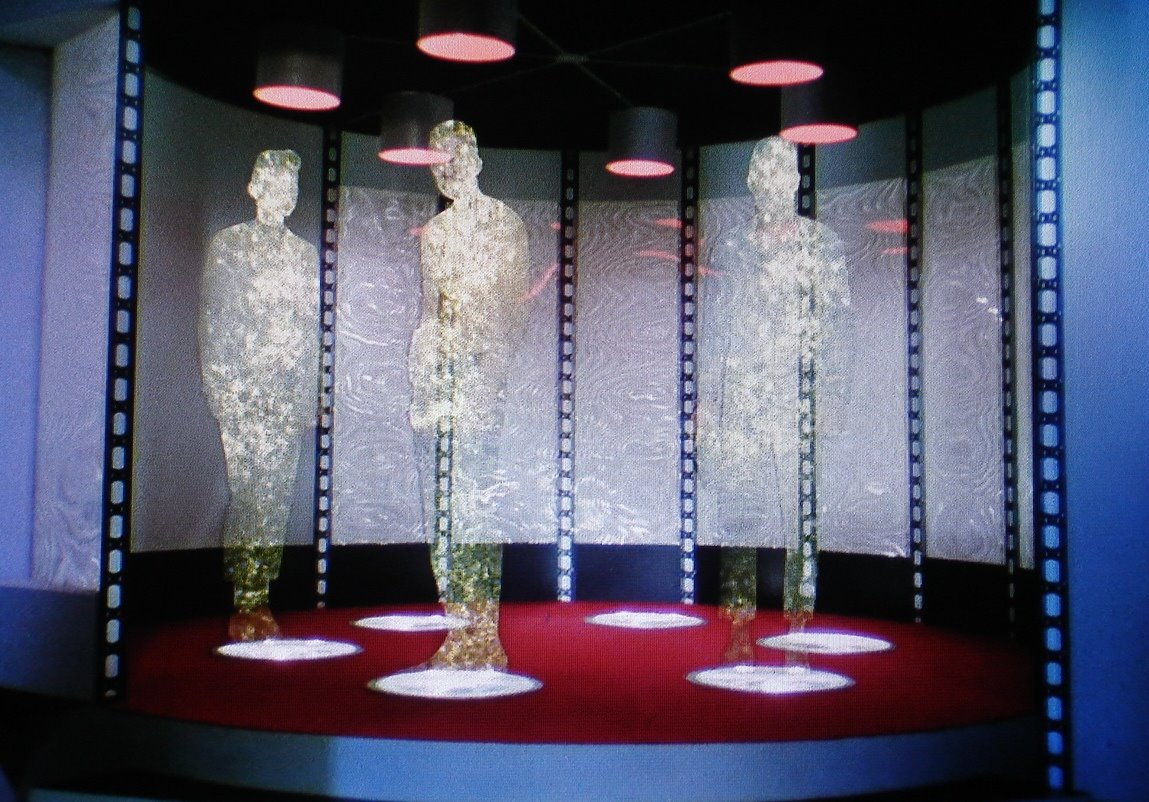
\includegraphics[width=0.4\textwidth]{images/beaming.jpg}
\end{center}

\end{frame}

\begin{frame}
\frametitle{Evaluation of Expressions}


The other option is a \alert{pipeline} which would allow us to immediately forward on the partial results from a particular operation.


\end{frame}

\begin{frame}
\frametitle{Materialization}

In the example from earlier where there is a three way join $r_{1} \bowtie r_{2} \bowtie r_{3}$ we will choose one of the ways to group this.

Then temporarily store the output in some temporary relation $r_{4}$ which is then used in the join with the third relation. 

\end{frame}

\begin{frame}
\frametitle{Compile This!}

Consider compilers!

When presented with a complex statement, we need to parse it and form a tree. 

Then, we work from the bottom level of the tree up to complete the expression. 

The code to be compiled is \texttt{ x = (y * 5) + z; }

\end{frame}

\begin{frame}
\frametitle{Low Level Operations}
In the database, we again, need to work on our low level operations and execute those operations (fetch rows, compute joins, whatever it is).

Then take the output and put this in a temporary relation. 

A temporary relation will be created at each step until all operations are complete. 

At that point we have the final result and can return it. 


\end{frame}

\begin{frame}
\frametitle{Materialization Has Costs}
The cost of materialization is the sum of the individual operations, plus the cost of writing all intermediate steps to disk. 

How large those intermediate costs are depends very heavily on how much data is to be written to disk at each step. 

However many tuples of each intermediate step fit into a block is important because it determines how many blocks are needed at each step. 
\end{frame}

\begin{frame}
\frametitle{Materialization Has Costs}


Once again, we get a hint that says if we get some choices about which operations to do sooner rather than later.

We want the ones that result in the fewest result tuples in the output relation...


\end{frame}

\begin{frame}
\frametitle{Pipelining}

The idea behind pipelining is to reduce or avoid the costs of storing those temporary files. 

Without pipelining, the first data item to finish stage 1 just kind of sits around waiting for the last item to finish stage 1 before the first item can start stage 2. 

It accordingly needs a place to wait. 

\end{frame}

\begin{frame}
\frametitle{Pipelining}
\begin{center}
	
\includegraphics[width=0.5\textwidth]{images/waiting.jpg}
\end{center}


Eliminating that place of waiting is the goal of pipelining.

\end{frame}

\begin{frame}
\frametitle{Types of Pipeline}

There are two approaches for how pipelines may execute. 

1. Demand-driven (or consumer-driven, pull) pipeline, the system requests at the output end the ``next'' chunk when it is ready to receive it.

2. Supply-driven (or producer-driven, push) pipeline, each stage of the pipeline is always trying to pick up the next chunk and process it.

\end{frame}

\begin{frame}
\frametitle{Think Producer-Consumer Problem}

A push-driven pipeline since it rather resembles the type of producer-consumer problem discussed in earlier courses. 

Each stage of the pipeline can be its own thread, and threads can be both a producer and a consumer.

Buffer sizes will be limited, of course, so there can be different stages that are blocked awaiting space in a buffer or waiting their turn to access a buffer


\end{frame}

\begin{frame}
\frametitle{Pipelining Problems}

The catch, when it comes to pipelining, is that there are some operations that don't work very well with it. 

Sorting is the most obvious example: you cannot send the first chunk of the sorted file on to the next stage until the entire file has been sorted. 

\begin{center}
	
\includegraphics[width=0.25\textwidth]{images/choppa.jpg}
\end{center}

\end{frame}

\begin{frame}
\frametitle{Pipelining Problems}

Our choice of evaluation algorithm for a select or join operation may also limit the ability to pipeline. 

These sorts of things are just limitations we cannot easily get around and may need to be accounted for in our plan for how to evaluate a query.


\end{frame}

\begin{frame}
\frametitle{Query Optimization}

The database server is responsible for choosing how to carry out the requested query and it is preferable to do it efficiently.

When we put some numbers to early examples, we saw that there can be orders of magnitude difference in how long it takes to execute a query. 

Conclusion: it is worth while for the database server to make the effort to decide what is optimal.


\end{frame}

\begin{frame}
\frametitle{Estimate Blocks}

We have looked at techniques for evaluation of how long we think a certain plan is going to take to execute.

They concentrated on how many disk operations we expected to take place. 

These typically included numbers like the number of tuples or blocks.

Question: how did we know how many tuples/blocks are in this relation?

\end{frame}


\begin{frame}
\frametitle{Use Metadata}

One way that might have immediately come to mind is the metadata kept by the database system. 

If it does provide us with some useful information like relation $r$ has 10592 tuples and is currently stored in 2591 blocks then we have some values to go on. 

\end{frame}


\begin{frame}
\frametitle{Use Metadata}

\begin{center}
	
\includegraphics[width=0.4\textwidth]{images/scorpio.jpg}
\end{center}

Those are the easy values to get. 

But how do we determine how many tuples we think will match the condition that some attribute $A$ is greater than some value $x$? 

And how many blocks will those tuples be in?


\end{frame}

\begin{frame}
\frametitle{Heuristics}
The answer lies mostly in \alert{heuristics}, or less charitably, educated guessing. 

A heuristic is a guideline or ``rule of thumb'' the gives us some hints. 

Suppose we know some statistics about $A$. If we do, then it can help us make some important decisions about what execution plans we choose. 


\end{frame}


\begin{frame}
\frametitle{Rule 1: Always Have Rules}
In fact, one of the main heuristic rules we should always try to follow is to cut down the size of intermediate relations whenever possible. 

That means select and project operations should be done early and certainly before a join. 

A join operation can result in a file size that is some multiple of the size of the input file so it is preferable to cut things down first.


\end{frame}


\begin{frame}
\frametitle{Tree Structure Map}
We previously introduced the idea of turning the input query into a tree structure which was then evaluated from the bottom up. 

We will often transform the input expression to a faster, better equivalent. 

\begin{center}
\includegraphics[width=0.7\textwidth]{images/optimization-1}
\end{center}


\end{frame}

\begin{frame}
\frametitle{Draw Up Battle Plans}

Depending on the nature of the query, 0, 1, or multiple equivalents may exist. 

It may be practical to write off some of those immediately, without assessing them, because we know they will be an inferior variant of a plan we have. 

The next step is then to draw up the plans for how we would execute the expressions. 

\begin{center}
\includegraphics[width=0.45\textwidth]{images/optimization-2}
\end{center}

\end{frame}


\begin{frame}
\frametitle{Don't Overthink This}

There may be many options for annotating each of the steps in the expression tree. 

A totally thorough approach would, once again, consider every possibility, but we realistically can eliminate some options. 

Then we may affix cost estimates to each plan as the sum of each part.

The final step is then to choose the the plan with the lowest cost.

\end{frame}

\begin{frame}
\frametitle{Tell Me Your Plan}

As a practical note, in SQL you may ask the database server to tell you how it would carry out a query. 

First you write the query as you normally would and prefix this query with the keyword \texttt{EXPLAIN}.


\end{frame}
\begin{frame}
\frametitle{EXPLAIN!!!!!}

\begin{center}
\includegraphics[width=0.9\textwidth]{images/EXPLAIN.png}
\end{center}


\end{frame}

\begin{frame}
\frametitle{Expression Transformation}

There are some rules for how exactly to transform a query to an equivalent alternative. 

These are a little bit like some things you may have learned in mathematics. 

We should remember that database operations do not, unless there is an explicit order-by clause, specify an order in which tuples appear in the output. 

Order does not matter in the output. 

\end{frame}

\begin{frame}
\frametitle{Notation Chart}

To spare a lot of repetition of what things mean, the notation will be centralized here. 

$\theta_{x}$ denotes a predicate (as part of a selection or join, for example).

$L_{x}$ denotes lists of attribute., 

$E$ denotes a relational algebra expression (a sub-expression or a relation $r$).

 All our other symbols from relational algebra remain the same as when they were first introduced.


\end{frame}

\begin{frame}
\frametitle{Rule 1: Conjunctive Selection}

Conjunctive selection can be turned into a sequence of individual selections.

Suppose we have a selection from address where province is ``ON'' and city is ``Kitchener''. 

We can do this as a selection on address where city is ``Kitchener'', producing a temporary relation. 

Then we do a selection where province is ``ON'' on that temporary relation. 

That is sometimes called a cascade of selection.

In relational algebra: $\sigma_{\theta_{1} \wedge \theta_{2}}(E) = \sigma_{\theta_{1}}(\sigma_{\theta_{2}}(E))$


\end{frame}


\begin{frame}
\frametitle{Rule 2: Selection Commutes}

Suppose the original selection is on address where city is ``Kitchener'', producing a temporary relation. 

Then we do a selection where province is ``ON'' on that temporary relation. 

This is equivalent to the opposite order, because the results are identical in both cases. 

In relational algebra: $\sigma_{\theta_{1}}(\sigma_{\theta_{2}}(E)) = \sigma_{\theta_{2}}(\sigma_{\theta_{1}}(E))$


\end{frame}

\begin{frame}
\frametitle{Rule 3: Projection Redundancy Elimination}

Only the last projection operation is needed. 

All other projection operations do not do anything. 

This should be pretty logical given that projection reduces the returned attributes to just those that are specified in the projection.

In relational algebra: $\Pi_{L_{1}}(\Pi_{L_{2}}(\Pi_{L_{3}}(E))) = \Pi_{L_{1}}(E)$

\end{frame}


\begin{frame}
\frametitle{Rule 4: Commuting Selection and Projection}

If a selection involves the same attributes as a projection list, we can commute the two operations. 

That is, if $L$ contains exactly the same set of attributes $A_{1}, A_{2}...$ that are referenced in $\theta$ then:

$\Pi_{L}(\sigma_{\theta}(E)) = \sigma_{\theta}(\Pi_{L}(E))$



\end{frame}

\begin{frame}
\frametitle{Rule 5: Selection Combination}

Selection may be combined with both cartesian product. 

This is, as you will recall, how a theta join works.

If a selection being combined with what is already a theta join, that is the same as a theta join with a conjunctive predicate/

a. $\sigma_{\theta}(E_{1} \times E_{2}) = E_{1} \bowtie_{\theta} E_{2}$

b. $\sigma_{\theta_{1}}( E_{1} \bowtie_{\theta_{2}} E_{2}) = E_{1} \bowtie_{\theta_{1}\wedge\theta_{2}} E_{2}$

\end{frame}

\begin{frame}
\frametitle{Rule 6: Theta Joins Commute}

Theta (and natural) joins commute, so the operands can be swapped in order and the same result is produced. 

That is a relief, considering our previous discussion of what blocks need to get moved into memory to complete the operation. 

This does potentially change the order of the attributes in the output, but we should not actually care.

\end{frame}


\begin{frame}
\frametitle{Rule 6: Theta Joins Commute}

Normally a selection statement, for example, specifies some attributes to be returned, meaning there is a projection operation to be done. 

If there is a select \texttt{*} operation, no order is guaranteed in the output anyway.

In relational algebra: $E_{1} \bowtie_{\theta} E_{2} = E_{2} \bowtie_{\theta} E_{1}$

The natural join is a special case of the theta join, so $E_{1} \bowtie E_{2} = E_{2} \bowtie E_{1}$

\end{frame}

\begin{frame}
\frametitle{Rule 7: Natural Join Associates}

When discussing joins, we actually already covered this rule, that they are associative. 

For theta joins, it looks a little more complicated, but the outcome is the same.


a. $(E_{1} \bowtie E_{2}) \bowtie E_{3} = E_{1} \bowtie (E_{2} \bowtie E_{3})$. 

b. $(E_{1} \bowtie_{\theta_{1}} E_{2}) \bowtie_{\theta_{2}\wedge\theta_{3}} E_{3} = E_{1} \bowtie_{\theta_{1}\wedge\theta_{3}} (E_{2} \bowtie_{\theta_{2}} E_{3})$. 

c. Because cartesian product is an empty theta join, $(E_{1} \times E_{2}) \times E_{3} = E_{1} \times (E_{2} \times E_{3})$. 

\end{frame}


\begin{frame}
\frametitle{Rule 8: Selection Distribution}

Selection distributes over theta join if the following conditions hold:

a. It distributes if all the attributes in $\theta_{0}$ involve only the attributes of one of the expressions $E$ being joined. 

 In this example, if $\theta_{0}$ applies only to $E_{1}$:

$\sigma_{\theta_{0}}(E_{1} \bowtie_{\theta} E_{2}) = (\sigma_{\theta_{0}}(E_{1})) \bowtie_{\theta} E_{2}$ 


\end{frame}

\begin{frame}
\frametitle{Rule 8: Selection Distribution}

b. It distributes when $\theta_{1}$ involves only the attributes of $E_{1}$ and $\theta_{2}$ only the attributes of $E_{2}$. 

This would mean cutting down both relations before performing the join.

$\sigma_{\theta_{1}\wedge\theta_{2}} (E_{1} \bowtie_{\theta} E_{2}) = (\sigma_{\theta_{1}}(E_{1})) \bowtie_{\theta} (\sigma_{\theta_{2}}(E_{2})) $

Both of these scenarios apply also for the cartesian product.

\end{frame}


\begin{frame}
\frametitle{Rule 9: Projection Distribution}

The projection operation can be distributed over theta join if the following conditions hold:

a. If $L_{1}$ and $L_{2}$ are attributes of $E_{1}$ and $E_{2}$ respectively, and $\theta$ contains only attributes in $L_{1} \cup L_{2}$, then we can distribute. 

$\Pi_{L_{1} \cup L_{2}}( E_{1} \bowtie_{\theta} E_{2} ) = (\Pi_{L_{1}}(E_{1})) \bowtie_{\theta} (\Pi_{L_{2}}(E_{2}))$

\end{frame}



\begin{frame}
\frametitle{Rule 9: Projection Distribution}

b. If $L_{1}$ and $L_{2}$ are attributes of $E_{1}$ and $E_{2}$ respectively, and $L_{3}$ are join attributes of $E_{1}$ not $L_{1} \cup L_{2}$ and $L_{4}$ are join attributes of $E_{2}$ not $L_{1} \cup L_{2}$:

$\Pi_{L_{1} \cup L_{2}} (E_{1} \bowtie_{\theta} E_{2}) = \Pi_{L_{1} \cup L_{2}}((\Pi_{L_{1} \cup L_{3}}(E1)) \bowtie_{\theta} (\Pi_{L_{2} \cup L_{4}}(E_{2})))$

Again, this can also be applied to cartesian product.


\end{frame}


\begin{frame}
\frametitle{Rule 10: Set Operations Commute}

The set operations union and intersection commute  (difference does not).

a. $E_{1} \cup E_{2} = E_{2} \cup E_{1}$

b. $E_{1} \cap E_{2} = E_{2} \cap E_{1}$


\end{frame}

\begin{frame}
\frametitle{Rule 11: Set Operations Associate}

Union and intersection are associative:

a. $(E_{1} \cup E_{2}) \cup E_{3} = E_{1} \cup (E_{2} \cup E_{3})$

b. $(E_{1} \cap E_{2}) \cap E_{3} = E_{1} \cap (E_{2} \cap E_{3})$

\end{frame}

\begin{frame}
\frametitle{Rule 12: Selection Distribution II}

Selection distributes over union, intersection, and difference operations:

a. $\sigma_{\theta}(E_{1} \cup E_{2}) = \sigma_{\theta}(E_{1}) \cup \sigma_{\theta}(E_{2})$

b. $\sigma_{\theta}(E_{1} \cap E_{2}) = \sigma_{\theta}(E_{1}) \cap \sigma_{\theta}(E_{2})$

c. $\sigma_{\theta}(E_{1} - E_{2}) = \sigma_{\theta}(E_{1}) - \sigma_{\theta}(E_{2})$



\end{frame}

\begin{frame}
\frametitle{Rule 13: Projection Distribution II }

The projection operation distributes over a union operation.

In relational algebra: $\Pi_{L}(E_{1} \cup E_{2} = (\Pi_{L}(E_{1}))\cup(\Pi_{L}(E_{2}))$



\end{frame}


\begin{frame}
\frametitle{Rules Review}


These rules are (sadly) neither a complete set nor minimal. 

There are other potential transformations that can be done, including various rules from boolean algebra (e.g., $\neg (a \wedge b) = \neg a \vee \neg b$)...


\end{frame}


\begin{frame}
\frametitle{Rules Review}


Having learned a bit about equivalence rules and what they are for, next time we will work on putting them to use and affixing cost estimates.

\begin{center}
	
\includegraphics[width=0.6\textwidth]{images/cost-estimates.jpg}
\end{center}

\end{frame}






\end{document}

